\def \hmina {\hspace{-0.1in}}
\def \hminb {\hspace{-0.2in}}

\def \fgw {2in}
\def \fgh {1in}

% \begin{floatingfigure}[r]{2in}  (and \end{..})

\begin{figure}[t]
    \centerline{
        % \hmina
        {\input{data/tradeoff-forward}}
        % \hminb
        %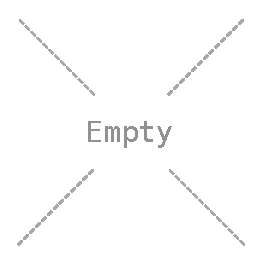
\includegraphics[height=\fgh]{empty.eps}
    }

    \mycaption{fig:eval-forward}{Forward I/O performance}{Median sequential I/O
    compared to baseline. Each cluster of 3 dots between configurations
    represents the 7:3, 5:5, and 3:7 ratios as discussed in
    \cref{subsec:eval-flexible}. Distance from baseline represents overhead.}
\end{figure}
